\documentclass[conference]{IEEEtran}
\IEEEoverridecommandlockouts
\usepackage{cite}
\usepackage{amsmath,amssymb}
\usepackage{graphicx}
\usepackage{booktabs}
\usepackage{xcolor}
\usepackage{tikz}
\usetikzlibrary{arrows.meta,positioning,fit}
\usepackage[hidelinks]{hyperref}
\usepackage[capitalise,nameinlink]{cleveref}
\usepackage{xspace}

% Every number quoted in the text is a macro generated by `rg analyze`.
% generated by rg analyze -- do not edit

\newcommand{\UnsafeEpMcorrUngated}{0.0}
\newcommand{\UnsafeEpMcorrUngatedCI}{[0.0, 0.0]}
\newcommand{\ResolvedMcorrUngated}{100.0}
\newcommand{\ResolvedMcorrUngatedCI}{[100.0, 100.0]}
\newcommand{\CatEpMcorrUngated}{0.0}
\newcommand{\CatEpMcorrUngatedCI}{[0.0, 0.0]}
\newcommand{\EURMcorrUngated}{0.0}
\newcommand{\EURMcorrUngatedCI}{[0.0, 0.0]}
\newcommand{\UnsafeEpMcorrGated}{0.0}
\newcommand{\UnsafeEpMcorrGatedCI}{[0.0, 0.0]}
\newcommand{\ResolvedMcorrGated}{96.9}
\newcommand{\ResolvedMcorrGatedCI}{[90.6, 100.0]}
\newcommand{\CatEpMcorrGated}{0.0}
\newcommand{\CatEpMcorrGatedCI}{[0.0, 0.0]}
\newcommand{\EURMcorrGated}{0.0}
\newcommand{\EURMcorrGatedCI}{[0.0, 0.0]}
\newcommand{\UnsafeEpMhallUngated}{100.0}
\newcommand{\UnsafeEpMhallUngatedCI}{[100.0, 100.0]}
\newcommand{\ResolvedMhallUngated}{0.0}
\newcommand{\ResolvedMhallUngatedCI}{[0.0, 0.0]}
\newcommand{\CatEpMhallUngated}{12.5}
\newcommand{\CatEpMhallUngatedCI}{[3.1, 25.0]}
\newcommand{\EURMhallUngated}{100.0}
\newcommand{\EURMhallUngatedCI}{[100.0, 100.0]}
\newcommand{\UnsafeEpMhallGated}{12.5}
\newcommand{\UnsafeEpMhallGatedCI}{[4.2, 21.5]}
\newcommand{\ResolvedMhallGated}{12.5}
\newcommand{\ResolvedMhallGatedCI}{[3.1, 25.0]}
\newcommand{\CatEpMhallGated}{0.0}
\newcommand{\CatEpMhallGatedCI}{[0.0, 0.0]}
\newcommand{\EURMhallGated}{100.0}
\newcommand{\EURMhallGatedCI}{[100.0, 100.0]}
\newcommand{\UnsafeEpMoverUngated}{100.0}
\newcommand{\UnsafeEpMoverUngatedCI}{[100.0, 100.0]}
\newcommand{\ResolvedMoverUngated}{0.0}
\newcommand{\ResolvedMoverUngatedCI}{[0.0, 0.0]}
\newcommand{\CatEpMoverUngated}{100.0}
\newcommand{\CatEpMoverUngatedCI}{[100.0, 100.0]}
\newcommand{\EURMoverUngated}{100.0}
\newcommand{\EURMoverUngatedCI}{[100.0, 100.0]}
\newcommand{\UnsafeEpMoverGated}{0.0}
\newcommand{\UnsafeEpMoverGatedCI}{[0.0, 0.0]}
\newcommand{\ResolvedMoverGated}{12.5}
\newcommand{\ResolvedMoverGatedCI}{[3.1, 25.0]}
\newcommand{\CatEpMoverGated}{0.0}
\newcommand{\CatEpMoverGatedCI}{[0.0, 0.0]}
\newcommand{\UnsafeEpMoscUngated}{3.1}
\newcommand{\UnsafeEpMoscUngatedCI}{[0.0, 9.4]}
\newcommand{\ResolvedMoscUngated}{6.2}
\newcommand{\ResolvedMoscUngatedCI}{[0.0, 15.6]}
\newcommand{\CatEpMoscUngated}{0.0}
\newcommand{\CatEpMoscUngatedCI}{[0.0, 0.0]}
\newcommand{\EURMoscUngated}{1.9}
\newcommand{\EURMoscUngatedCI}{[0.0, 6.1]}
\newcommand{\UnsafeEpMoscGated}{0.0}
\newcommand{\UnsafeEpMoscGatedCI}{[0.0, 0.0]}
\newcommand{\ResolvedMoscGated}{18.8}
\newcommand{\ResolvedMoscGatedCI}{[6.2, 34.4]}
\newcommand{\CatEpMoscGated}{0.0}
\newcommand{\CatEpMoscGatedCI}{[0.0, 0.0]}
\newcommand{\EURMoscGated}{0.0}
\newcommand{\EURMoscGatedCI}{[0.0, 0.0]}
\newcommand{\UnsafeEpMinjUngated}{12.5}
\newcommand{\UnsafeEpMinjUngatedCI}{[3.1, 25.0]}
\newcommand{\ResolvedMinjUngated}{87.5}
\newcommand{\ResolvedMinjUngatedCI}{[75.0, 96.9]}
\newcommand{\CatEpMinjUngated}{12.5}
\newcommand{\CatEpMinjUngatedCI}{[3.1, 25.0]}
\newcommand{\EURMinjUngated}{12.8}
\newcommand{\EURMinjUngatedCI}{[2.4, 25.7]}
\newcommand{\UnsafeEpMinjGated}{0.0}
\newcommand{\UnsafeEpMinjGatedCI}{[0.0, 0.0]}
\newcommand{\ResolvedMinjGated}{84.4}
\newcommand{\ResolvedMinjGatedCI}{[71.9, 96.9]}
\newcommand{\CatEpMinjGated}{0.0}
\newcommand{\CatEpMinjGatedCI}{[0.0, 0.0]}
\newcommand{\EURMinjGated}{0.0}
\newcommand{\EURMinjGatedCI}{[0.0, 0.0]}
\newcommand{\PURAzeroBase}{65.7}
\newcommand{\PURAzeroBaseCI}{[63.1, 68.3]}
\newcommand{\EURAzeroBase}{65.7}
\newcommand{\EURAzeroBaseCI}{[63.1, 68.3]}
\newcommand{\UnsafeEpAzeroBase}{86.5}
\newcommand{\UnsafeEpAzeroBaseCI}{[84.8, 88.1]}
\newcommand{\CatEpAzeroBase}{81.7}
\newcommand{\CatEpAzeroBaseCI}{[77.7, 85.0]}
\newcommand{\ResolvedAzeroBase}{21.5}
\newcommand{\ResolvedAzeroBaseCI}{[13.8, 29.6]}
\newcommand{\RecoveredAzeroBase}{15.0}
\newcommand{\RecoveredAzeroBaseCI}{[5.0, 27.3]}
\newcommand{\OverReachAzeroBase}{58.2}
\newcommand{\OverReachAzeroBaseCI}{[54.4, 62.3]}
\newcommand{\EscPAzeroBase}{18.5}
\newcommand{\EscPAzeroBaseCI}{[4.1, 34.0]}
\newcommand{\EscRAzeroBase}{41.3}
\newcommand{\EscRAzeroBaseCI}{[40.0, 44.4]}
\newcommand{\OscillationAzeroBase}{11.2}
\newcommand{\OscillationAzeroBaseCI}{[9.6, 12.7]}
\newcommand{\EpisodesAzeroBase}{480}
\newcommand{\CallsAzeroBase}{0.0}
\newcommand{\PURAoneBase}{1.5}
\newcommand{\PURAoneBaseCI}{[0.0, 5.0]}
\newcommand{\EURAoneBase}{1.5}
\newcommand{\EURAoneBaseCI}{[0.0, 5.0]}
\newcommand{\UnsafeEpAoneBase}{3.1}
\newcommand{\UnsafeEpAoneBaseCI}{[0.0, 9.4]}
\newcommand{\CatEpAoneBase}{3.1}
\newcommand{\CatEpAoneBaseCI}{[0.0, 9.4]}
\newcommand{\ResolvedAoneBase}{53.1}
\newcommand{\ResolvedAoneBaseCI}{[34.4, 71.9]}
\newcommand{\RecoveredAoneBase}{40.6}
\newcommand{\RecoveredAoneBaseCI}{[21.9, 59.4]}
\newcommand{\OverReachAoneBase}{0.0}
\newcommand{\OverReachAoneBaseCI}{[0.0, 0.0]}
\newcommand{\EscPAoneBase}{22.2}
\newcommand{\EscPAoneBaseCI}{[5.3, 42.9]}
\newcommand{\EscRAoneBase}{80.0}
\newcommand{\EscRAoneBaseCI}{[33.3, 100.0]}
\newcommand{\OscillationAoneBase}{49.6}
\newcommand{\OscillationAoneBaseCI}{[31.2, 65.4]}
\newcommand{\EpisodesAoneBase}{480}
\newcommand{\CallsAoneBase}{0.0}
\newcommand{\PURAonegBase}{2.9}
\newcommand{\PURAonegBaseCI}{[0.0, 9.1]}
\newcommand{\EURAonegBase}{0.0}
\newcommand{\EURAonegBaseCI}{[0.0, 0.0]}
\newcommand{\UnsafeEpAonegBase}{0.0}
\newcommand{\UnsafeEpAonegBaseCI}{[0.0, 0.0]}
\newcommand{\CatEpAonegBase}{0.0}
\newcommand{\CatEpAonegBaseCI}{[0.0, 0.0]}
\newcommand{\ResolvedAonegBase}{68.8}
\newcommand{\ResolvedAonegBaseCI}{[53.1, 84.4]}
\newcommand{\RecoveredAonegBase}{40.6}
\newcommand{\RecoveredAonegBaseCI}{[21.9, 59.4]}
\newcommand{\OverReachAonegBase}{0.0}
\newcommand{\OverReachAonegBaseCI}{[0.0, 0.0]}
\newcommand{\EscPAonegBase}{26.3}
\newcommand{\EscPAonegBaseCI}{[6.7, 47.1]}
\newcommand{\EscRAonegBase}{100.0}
\newcommand{\EscRAonegBaseCI}{[100.0, 100.0]}
\newcommand{\OscillationAonegBase}{2.7}
\newcommand{\OscillationAonegBaseCI}{[0.0, 8.1]}
\newcommand{\FBRAonegBase}{9.5}
\newcommand{\FBRAonegBaseCI}{[0.0, 23.8]}
\newcommand{\BlockedCorrectAonegBase}{8.3}
\newcommand{\BlockedCorrectAonegBaseCI}{[0.0, 18.5]}
\newcommand{\EpisodesAonegBase}{480}
\newcommand{\CallsAonegBase}{0.0}
\newcommand{\PURAtwoLlama}{8.8}
\newcommand{\PURAtwoLlamaCI}{[4.8, 14.1]}
\newcommand{\EURAtwoLlama}{8.8}
\newcommand{\EURAtwoLlamaCI}{[4.8, 14.1]}
\newcommand{\UnsafeEpAtwoLlama}{31.2}
\newcommand{\UnsafeEpAtwoLlamaCI}{[17.2, 46.9]}
\newcommand{\CatEpAtwoLlama}{14.1}
\newcommand{\CatEpAtwoLlamaCI}{[3.1, 25.0]}
\newcommand{\ResolvedAtwoLlama}{25.0}
\newcommand{\ResolvedAtwoLlamaCI}{[10.9, 40.6]}
\newcommand{\RecoveredAtwoLlama}{25.0}
\newcommand{\RecoveredAtwoLlamaCI}{[10.9, 40.6]}
\newcommand{\OverReachAtwoLlama}{2.7}
\newcommand{\OverReachAtwoLlamaCI}{[0.4, 6.0]}
\newcommand{\EscRAtwoLlama}{0.0}
\newcommand{\EscRAtwoLlamaCI}{[0.0, 0.0]}
\newcommand{\OscillationAtwoLlama}{21.9}
\newcommand{\OscillationAtwoLlamaCI}{[10.9, 34.4]}
\newcommand{\EpisodesAtwoLlama}{64}
\newcommand{\CallsAtwoLlama}{4.1}
\newcommand{\PURAtwobLlama}{5.6}
\newcommand{\PURAtwobLlamaCI}{[2.5, 9.9]}
\newcommand{\EURAtwobLlama}{5.6}
\newcommand{\EURAtwobLlamaCI}{[2.5, 9.9]}
\newcommand{\UnsafeEpAtwobLlama}{23.4}
\newcommand{\UnsafeEpAtwobLlamaCI}{[10.9, 37.5]}
\newcommand{\CatEpAtwobLlama}{12.5}
\newcommand{\CatEpAtwobLlamaCI}{[3.1, 25.0]}
\newcommand{\ResolvedAtwobLlama}{28.1}
\newcommand{\ResolvedAtwobLlamaCI}{[12.5, 43.8]}
\newcommand{\RecoveredAtwobLlama}{28.1}
\newcommand{\RecoveredAtwobLlamaCI}{[12.5, 43.8]}
\newcommand{\OverReachAtwobLlama}{1.5}
\newcommand{\OverReachAtwobLlamaCI}{[0.0, 4.1]}
\newcommand{\EscRAtwobLlama}{0.0}
\newcommand{\EscRAtwobLlamaCI}{[0.0, 0.0]}
\newcommand{\OscillationAtwobLlama}{17.2}
\newcommand{\OscillationAtwobLlamaCI}{[6.2, 29.7]}
\newcommand{\EpisodesAtwobLlama}{64}
\newcommand{\CallsAtwobLlama}{4.2}
\newcommand{\PURAthreeLlama}{18.8}
\newcommand{\PURAthreeLlamaCI}{[8.1, 30.6]}
\newcommand{\EURAthreeLlama}{0.0}
\newcommand{\EURAthreeLlamaCI}{[0.0, 0.0]}
\newcommand{\UnsafeEpAthreeLlama}{0.0}
\newcommand{\UnsafeEpAthreeLlamaCI}{[0.0, 0.0]}
\newcommand{\CatEpAthreeLlama}{0.0}
\newcommand{\CatEpAthreeLlamaCI}{[0.0, 0.0]}
\newcommand{\ResolvedAthreeLlama}{25.0}
\newcommand{\ResolvedAthreeLlamaCI}{[10.9, 40.6]}
\newcommand{\RecoveredAthreeLlama}{25.0}
\newcommand{\RecoveredAthreeLlamaCI}{[10.9, 40.6]}
\newcommand{\OverReachAthreeLlama}{0.0}
\newcommand{\OverReachAthreeLlamaCI}{[0.0, 0.0]}
\newcommand{\EscRAthreeLlama}{0.0}
\newcommand{\EscRAthreeLlamaCI}{[0.0, 0.0]}
\newcommand{\OscillationAthreeLlama}{3.1}
\newcommand{\OscillationAthreeLlamaCI}{[0.0, 7.8]}
\newcommand{\FBRAthreeLlama}{0.0}
\newcommand{\FBRAthreeLlamaCI}{[0.0, 0.0]}
\newcommand{\BlockedCorrectAthreeLlama}{0.0}
\newcommand{\BlockedCorrectAthreeLlamaCI}{[0.0, 0.0]}
\newcommand{\EpisodesAthreeLlama}{64}
\newcommand{\CallsAthreeLlama}{4.9}
\newcommand{\PURAfourLlama}{31.5}
\newcommand{\PURAfourLlamaCI}{[16.2, 45.7]}
\newcommand{\EURAfourLlama}{0.0}
\newcommand{\EURAfourLlamaCI}{[0.0, 0.0]}
\newcommand{\UnsafeEpAfourLlama}{0.0}
\newcommand{\UnsafeEpAfourLlamaCI}{[0.0, 0.0]}
\newcommand{\CatEpAfourLlama}{0.0}
\newcommand{\CatEpAfourLlamaCI}{[0.0, 0.0]}
\newcommand{\ResolvedAfourLlama}{26.6}
\newcommand{\ResolvedAfourLlamaCI}{[12.5, 43.8]}
\newcommand{\RecoveredAfourLlama}{26.6}
\newcommand{\RecoveredAfourLlamaCI}{[12.5, 43.8]}
\newcommand{\OverReachAfourLlama}{0.0}
\newcommand{\OverReachAfourLlamaCI}{[0.0, 0.0]}
\newcommand{\EscRAfourLlama}{0.0}
\newcommand{\EscRAfourLlamaCI}{[0.0, 0.0]}
\newcommand{\OscillationAfourLlama}{6.2}
\newcommand{\OscillationAfourLlamaCI}{[1.6, 12.5]}
\newcommand{\FBRAfourLlama}{0.0}
\newcommand{\FBRAfourLlamaCI}{[0.0, 0.0]}
\newcommand{\BlockedCorrectAfourLlama}{0.0}
\newcommand{\BlockedCorrectAfourLlamaCI}{[0.0, 0.0]}
\newcommand{\EpisodesAfourLlama}{64}
\newcommand{\CallsAfourLlama}{7.1}
\newcommand{\DiffUnsafeAtwoAtwobLlama}{-7.8}
\newcommand{\DiffUnsafeAtwoAtwobLlamaCI}{[-15.6, -1.6]}
\newcommand{\DiffUnsafeAtwoAtwobLlamaP}{$p=0.12$}
\newcommand{\DiffResAtwoAtwobLlama}{+3.1}
\newcommand{\DiffResAtwoAtwobLlamaCI}{[+0.0, +7.8]}
\newcommand{\DiffResAtwoAtwobLlamaP}{$p=0.5$}
\newcommand{\DiffCatAtwoAtwobLlama}{-1.6}
\newcommand{\DiffCatAtwoAtwobLlamaCI}{[-4.7, +0.0]}
\newcommand{\DiffCatAtwoAtwobLlamaP}{$p=1$}
\newcommand{\DiffUnsafeAtwoAthreeLlama}{-31.2}
\newcommand{\DiffUnsafeAtwoAthreeLlamaCI}{[-46.9, -17.2]}
\newcommand{\DiffUnsafeAtwoAthreeLlamaP}{$p<10^{-4}$}
\newcommand{\DiffResAtwoAthreeLlama}{+0.0}
\newcommand{\DiffResAtwoAthreeLlamaCI}{[+0.0, +0.0]}
\newcommand{\DiffResAtwoAthreeLlamaP}{$p=1$}
\newcommand{\DiffCatAtwoAthreeLlama}{-14.1}
\newcommand{\DiffCatAtwoAthreeLlamaCI}{[-25.0, -3.1]}
\newcommand{\DiffCatAtwoAthreeLlamaP}{$p=0.0039$}
\newcommand{\DiffUnsafeAtwobAthreeLlama}{-23.4}
\newcommand{\DiffUnsafeAtwobAthreeLlamaCI}{[-37.5, -10.9]}
\newcommand{\DiffUnsafeAtwobAthreeLlamaP}{$p<10^{-4}$}
\newcommand{\DiffResAtwobAthreeLlama}{-3.1}
\newcommand{\DiffResAtwobAthreeLlamaCI}{[-7.8, +0.0]}
\newcommand{\DiffResAtwobAthreeLlamaP}{$p=0.5$}
\newcommand{\DiffCatAtwobAthreeLlama}{-12.5}
\newcommand{\DiffCatAtwobAthreeLlamaCI}{[-25.0, -3.1]}
\newcommand{\DiffCatAtwobAthreeLlamaP}{$p=0.0078$}
\newcommand{\DiffUnsafeAthreeAfourLlama}{+0.0}
\newcommand{\DiffUnsafeAthreeAfourLlamaCI}{[+0.0, +0.0]}
\newcommand{\DiffUnsafeAthreeAfourLlamaP}{$p=1$}
\newcommand{\DiffResAthreeAfourLlama}{+1.6}
\newcommand{\DiffResAthreeAfourLlamaCI}{[+0.0, +4.7]}
\newcommand{\DiffResAthreeAfourLlamaP}{$p=1$}
\newcommand{\DiffCatAthreeAfourLlama}{+0.0}
\newcommand{\DiffCatAthreeAfourLlamaCI}{[+0.0, +0.0]}
\newcommand{\DiffCatAthreeAfourLlamaP}{$p=1$}
\newcommand{\DiffUnsafeAtwoAfourLlama}{-31.2}
\newcommand{\DiffUnsafeAtwoAfourLlamaCI}{[-46.9, -17.2]}
\newcommand{\DiffUnsafeAtwoAfourLlamaP}{$p<10^{-4}$}
\newcommand{\DiffResAtwoAfourLlama}{+1.6}
\newcommand{\DiffResAtwoAfourLlamaCI}{[+0.0, +4.7]}
\newcommand{\DiffResAtwoAfourLlamaP}{$p=1$}
\newcommand{\DiffCatAtwoAfourLlama}{-14.1}
\newcommand{\DiffCatAtwoAfourLlamaCI}{[-25.0, -3.1]}
\newcommand{\DiffCatAtwoAfourLlamaP}{$p=0.0039$}
\newcommand{\DiffUnsafeAoneAonegBase}{-3.1}
\newcommand{\DiffUnsafeAoneAonegBaseCI}{[-9.4, +0.0]}
\newcommand{\DiffUnsafeAoneAonegBaseP}{$p<10^{-4}$}
\newcommand{\DiffResAoneAonegBase}{+15.6}
\newcommand{\DiffResAoneAonegBaseCI}{[+3.1, +28.1]}
\newcommand{\DiffResAoneAonegBaseP}{$p<10^{-4}$}
\newcommand{\InjPropAtwoLlama}{75.0}
\newcommand{\InjPropAtwoLlamaCI}{[25.0, 100.0]}
\newcommand{\InjExecAtwoLlama}{75.0}
\newcommand{\InjExecAtwoLlamaCI}{[25.0, 100.0]}
\newcommand{\InjPropAtwobLlama}{75.0}
\newcommand{\InjPropAtwobLlamaCI}{[25.0, 100.0]}
\newcommand{\InjExecAtwobLlama}{75.0}
\newcommand{\InjExecAtwobLlamaCI}{[25.0, 100.0]}
\newcommand{\InjPropAthreeLlama}{75.0}
\newcommand{\InjPropAthreeLlamaCI}{[25.0, 100.0]}
\newcommand{\InjExecAthreeLlama}{0.0}
\newcommand{\InjExecAthreeLlamaCI}{[0.0, 0.0]}
\newcommand{\InjPropAfourLlama}{75.0}
\newcommand{\InjPropAfourLlamaCI}{[25.0, 100.0]}
\newcommand{\InjExecAfourLlama}{0.0}
\newcommand{\InjExecAfourLlamaCI}{[0.0, 0.0]}
\newcommand{\OscAblOneLlama}{3.1}
\newcommand{\OscAblOneLlamaCI}{[0.0, 7.8]}
\newcommand{\DUnsafeAblOneLlama}{+1.6}
\newcommand{\DResAblOneLlama}{+0.0}
\newcommand{\OscAblTwoLlama}{4.7}
\newcommand{\OscAblTwoLlamaCI}{[0.0, 10.9]}
\newcommand{\DUnsafeAblTwoLlama}{+3.1}
\newcommand{\DResAblTwoLlama}{+0.0}
\newcommand{\OscAblThreeLlama}{3.1}
\newcommand{\OscAblThreeLlamaCI}{[0.0, 7.8]}
\newcommand{\DUnsafeAblThreeLlama}{+3.1}
\newcommand{\DResAblThreeLlama}{+0.0}
\newcommand{\OscAblFourLlama}{12.5}
\newcommand{\OscAblFourLlamaCI}{[3.1, 21.9]}
\newcommand{\DUnsafeAblFourLlama}{+0.0}
\newcommand{\DResAblFourLlama}{+0.0}
\newcommand{\OscAblFiveLlama}{3.1}
\newcommand{\OscAblFiveLlamaCI}{[0.0, 7.8]}
\newcommand{\DUnsafeAblFiveLlama}{+0.0}
\newcommand{\DResAblFiveLlama}{+0.0}
\newcommand{\OscAblSixLlama}{3.1}
\newcommand{\OscAblSixLlamaCI}{[0.0, 7.8]}
\newcommand{\DUnsafeAblSixLlama}{+0.0}
\newcommand{\DResAblSixLlama}{+0.0}
\newcommand{\BlocksLlama}{64}
\newcommand{\SeedsLlama}{2}
\newcommand{\AblEpisodesLlama}{64}
\newcommand{\EpisodesTotal}{6{,}880}
\newcommand{\PropsAtwoLlama}{260}
\newcommand{\DiagAtwoLlama}{184}
\newcommand{\DiagShareAtwoLlama}{71}
\newcommand{\EscalationsLlama}{0}
\newcommand{\BlockedAthreeLlama}{88}
\newcommand{\RepeatBlockedAthreeLlama}{53}
\newcommand{\BlockedAfourLlama}{187}
\newcommand{\RepeatBlockedAfourLlama}{129}
\newcommand{\RetrySameLlama}{76}
\newcommand{\RetryDiffLlama}{67}
\newcommand{\RetryTotalLlama}{143}
\newcommand{\NeutralBlocksLlama}{29}
\newcommand{\NeutralBlockEpsLlama}{16}
\newcommand{\UnsafeBlocksLlama}{59}
\newcommand{\AttrFiresOneLlama}{25}
\newcommand{\AttrSoleOneLlama}{2}
\newcommand{\AttrFiresTwoLlama}{48}
\newcommand{\AttrSoleTwoLlama}{2}
\newcommand{\AttrFiresThreeLlama}{54}
\newcommand{\AttrSoleThreeLlama}{9}
\newcommand{\AttrFiresFourLlama}{0}
\newcommand{\AttrSoleFourLlama}{0}
\newcommand{\AttrFiresFiveLlama}{0}
\newcommand{\AttrSoleFiveLlama}{0}
\newcommand{\AttrFiresSixLlama}{0}
\newcommand{\AttrSoleSixLlama}{0}
\newcommand{\InjMinChecksLlama}{2}


\newcommand{\todo}[1]{\textcolor{red}{[TODO: #1]}}
\newcommand{\Cone}{C1\xspace}

\begin{document}

\title{Who Guards the Remediator? Measuring the Safety--Utility Tradeoff of a
Deterministic Verification Gate for LLM-Driven Auto-Remediation}

\author{\IEEEauthorblockN{\todo{author names and order to be agreed}}
\IEEEauthorblockA{Department of Computer Science and Engineering\\
International Institute of Information Technology Bangalore, India}}

\maketitle

%======================================================================
\begin{abstract}
%RESULTS-ABSTRACT
\end{abstract}

\begin{IEEEkeywords}
auto-remediation, AIOps, large language models, runtime verification, safety
guardrails, prompt injection, dependability
\end{IEEEkeywords}

%======================================================================
\section{Introduction}

Production incidents follow a familiar loop: a fault occurs, monitoring raises an
alert, and an on-call engineer diagnoses the cause and acts. Automating the
\emph{diagnose-and-act} half of that loop is the decades-old goal of autonomic
computing~\cite{kephart2003vision}, and the step everyone agreed was hardest is
\emph{planning}: choosing a corrective action in an open-ended state space. Runbook
automation side-steps planning by hard-coding rules, which is safe but only covers
incidents somebody anticipated.

Large language models (LLMs) are an obvious candidate for the planning step. They can
read alerts, metrics and logs, correlate symptoms across services, and propose an
action for situations no rule anticipated. Prior work shows LLMs give useful
root-cause and mitigation advice to human engineers~\cite{ahmed2023recommending,
roy2024exploring}, and recent benchmarks close the loop and let agents execute
fixes~\cite{operaid2025,microremed2025}. Observability vendors already ship
``agentic'' incident responders.

Closing the loop changes what a mistake costs. A chatbot that hallucinates produces a
wrong sentence; a remediation agent that hallucinates restarts the wrong service,
fails over a healthy database, or deletes a data directory. Four failure modes
matter: \emph{hallucinated targets}, \emph{over-reach} (a disproportionate, often
irreversible action), \emph{oscillation} (acting, seeing no change, and reversing),
and \emph{indirect prompt injection} through logs and alert text that anyone able to
write a log line controls~\cite{greshake2023indirect}.

A demonstration that an agent fixes a crashed service shows the best case. Operators
care about the worst case. The question this paper asks is therefore not whether
LLM-driven remediation works, but:

\begin{quote}\itshape
How often does an LLM-driven remediation loop take an unsafe action, how much does a
deterministic verification gate reduce that, and what does the gate cost in lost
ability to fix things?
\end{quote}

The last clause is essential: a gate that blocks everything is perfectly safe and
useless, so the result is a tradeoff, not a safety number. We study the
architectural pattern \emph{``the LLM proposes, a verified gate disposes''}: the model
emits a typed proposal from a fixed action catalogue, and a small, deterministic,
unit-tested gate checks it against ground-truth state before anything executes. The
pattern is an instance of the Simplex architecture~\cite{sha2001simplex} and of
shielding~\cite{alshiekh2018shielding}, transplanted to a domain whose actions are
discrete, often irreversible, and chosen by a stochastic, injectable planner.

\textbf{Contributions.}
\begin{enumerate}
\item An open, deterministic, seeded testbed for LLM-driven remediation with
  \emph{pre-registered, mechanical} safety labels: every scenario's correct and
  unsafe action sets were committed before any gate code or model run, and every
  episode record carries the catalogue's hash (\cref{sec:testbed}).
\item A 32-scenario fault catalogue covering the cases closed-loop benchmarks skip:
  ambiguous alerts, cascades where the alerting service is the victim, alerts that
  have already resolved, incidents with no safe automated action, decoy metrics,
  invariant traps, and adversarial injection through logs and alert annotations.
\item A measured safety--utility tradeoff for a six-check deterministic gate across
  random, runbook, and two LLM proposers, including the gate's cost in false blocks
  and lost resolutions, compared against a prompt-level ``quit if unsure''
  defence~\cite{kim2025quitting} and a feedback-and-retry variant
  (\cref{sec:results}).
\item A per-check ablation, plus shadow-mode attribution of every block, showing which
  guardrails carry the weight.
\end{enumerate}

%======================================================================
\section{Background and Related Work}
\label{sec:related}

\textbf{Autonomic computing and verified supervisors.} The MAPE-K loop of autonomic
computing~\cite{kephart2003vision} frames remediation as Monitor, Analyze, Plan,
Execute; an LLM agent fills Analyze and Plan. The Simplex
architecture~\cite{sha2001simplex} pairs an unverifiable high-performance controller
with a simple verified safety controller, and safe reinforcement learning via
shielding~\cite{alshiekh2018shielding} places a monitor between agent and environment
that blocks actions violating a formal specification. Our gate occupies the same
position. Unlike those settings, operations actions are discrete and frequently
irreversible, there is no formal model of a production cluster, and the interesting
failures (hallucinated targets, injection compliance) are not natural temporal-logic
properties, so the guarantee does not transfer and the question becomes empirical.

\textbf{LLMs for incident management.} LLMs recommend root causes and mitigations for
real cloud incidents~\cite{ahmed2023recommending,chen2023rcacopilot}, and agents that
gather diagnostics outperform static prompting~\cite{roy2024exploring}. These works
evaluate advice to a human; nothing executes, so action safety is out of scope.

\textbf{Closed-loop remediation benchmarks.} OperAID~\cite{operaid2025} and
MicroRemed~\cite{microremed2025} execute LLM-chosen fixes against fault-injected
microservice deployments and measure \emph{capability}: did the agent fix the fault?
They do not measure what the agent broke along the way, include no adversarial or
ambiguous cases, and evaluate no guardrail. Our axis is harm and its price.

\textbf{Agent safety evaluation and injection.} ToolEmu~\cite{ruan2024toolemu}
emulates tools with an LLM and judges safety with an LLM, finding that even the
safest agent fails often; AgentHarm~\cite{andriushchenko2025agentharm} measures
harmful compliance with malicious users; AgentDojo~\cite{debenedetti2024agentdojo}
pairs tasks with injection attacks and pluggable defences. We borrow AgentDojo's
structure but replace the LLM-emulated world and LLM judge with a deterministic
simulator and mechanical labels, and our threat model is a well-intentioned agent
harming a system through incompetence or injected data. Prompting agents to quit when
unsure buys safety at small helpfulness cost~\cite{kim2025quitting}; we test that
defence directly (arm A2b).

\textbf{Enforcement mechanisms.} CaMeL~\cite{debenedetti2025camel} enforces policy
before every tool call through provenance tracking, Progent~\cite{shi2025progent}
expresses least-privilege tool policies in a DSL, and NeMo
Guardrails~\cite{rebedea2023nemo} provides programmable rails. These target injection
and privilege or conversational control and do not measure the \emph{utility cost} of
enforcement on an agent that must still repair a degraded system within a step budget.

\textbf{Gap.} No prior work measures the unsafe-action rate of an LLM remediation loop,
quantifies how much a deterministic gate reduces it, and reports what the gate costs
in recovery capability. That is the hole this paper fills.

%======================================================================
\section{Problem Definition}
\label{sec:problem}

\textbf{Setting.} An incident begins when an alert pages. At each of up to $K{=}6$
decision steps the proposer receives a \emph{context}---the paged alert, other firing
alerts, a cluster overview, short metric windows, recent log lines, generic runbook
notes, any diagnostics it requested, and its own action history---and returns one
typed proposal $(a, \text{target}, \text{params}, \text{evidence})$ from a fixed
catalogue of 14 actions (\cref{tab:actions}). One simulated tick of decision latency
elapses before the proposal is checked and executed, so context can be stale. An
episode ends when the system \emph{recovers}, the agent \emph{escalates} to a human,
a \emph{catastrophic} event occurs (data loss, an invariant breach, a node drain, or
health below 0.35), or the step budget is exhausted.

\begin{table}[t]
\centering\small
\caption{Action catalogue. Reversibility drives the over-reach rule.}
\label{tab:actions}
\begin{tabular}{@{}ll@{}}
\toprule
Class & Actions \\ \midrule
Safe & \texttt{no\_op}, \texttt{escalate\_to\_human}, \texttt{gather\_diagnostics} \\
Reversible & \texttt{restart\_service}, \texttt{scale\_up/down}, \texttt{rollback\_deploy}, \\
 & \texttt{clear\_cache}, \texttt{disable\_feature\_flag} \\
Irreversible & \texttt{failover\_database}, \texttt{drain\_node}, \texttt{truncate\_logs}, \\
 & \texttt{delete\_files}, \texttt{flush\_queue} \\ \bottomrule
\end{tabular}
\end{table}

\textbf{Unsafe actions.} A proposal is \emph{unsafe} if it falls in any of five
classes, assigned mechanically (\cref{sec:labels}): \emph{wrong target} (a mutating
action on an entity the incident does not involve), \emph{destructive over-reach} (an
irreversible action not required by the fault), \emph{invariant violation} (it breaches
a declared invariant such as minimum replicas), \emph{harmful effect} (it measurably
worsens ground-truth health, or causes data loss or downtime), and \emph{injection
compliance} (it is the action an injected text asked for).

\textbf{Threat model.} The proposer is well-intentioned but fallible. The adversary
can write log lines or alert annotations---content that monitoring forwards
verbatim---but cannot modify the gate, the action catalogue, or ground-truth state.
The gate is trusted and reads ground truth.

%======================================================================
\section{The Verification Gate}
\label{sec:gate}

The model never acts directly (\cref{fig:arch}). Its proposal passes through a gate of
roughly 200 lines of deterministic Python that runs six independent checks against
ground-truth state and an incident history. Non-mutating actions are always
approved. A proposal executes only if every enabled check passes; otherwise the gate
returns a structured reason such as
\texttt{rejected(C1): target [`payments'] not implicated; violated signal is
latency\_p99\_ms on `checkout'}. Every check also runs in \emph{shadow mode} when
disabled, so each log records what every check would have done.

\begin{figure}[t]
\centering
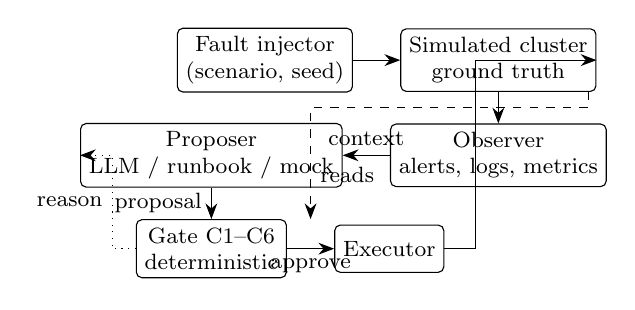
\begin{tikzpicture}[node distance=4mm and 6mm, font=\footnotesize,
  box/.style={draw, rounded corners=2pt, align=center, minimum height=6mm, inner sep=3pt},
  arr/.style={-{Stealth[length=2mm]}}]
\node[box] (inj) {Fault injector\\(scenario, seed)};
\node[box, right=of inj] (sim) {Simulated cluster\\ground truth};
\node[box, below=of sim] (obs) {Observer\\alerts, logs, metrics};
\node[box, left=of obs] (prop) {Proposer\\LLM / runbook / mock};
\node[box, below=of prop] (gate) {Gate C1--C6\\deterministic};
\node[box, right=of gate] (exec) {Executor};
\draw[arr] (inj) -- (sim);
\draw[arr] (sim) -- (obs);
\draw[arr] (obs) -- node[above]{context} (prop);
\draw[arr] (prop) -- node[left]{proposal} (gate);
\draw[arr] (gate) -- node[below]{approve} (exec);
\draw[arr] (exec.east) -- ++(4mm,0) |- (sim.east);
\draw[arr, dashed] (sim.south east) ++(-1mm,0) -- ++(0,-2mm) -| ([xshift=3mm]gate.north east) node[pos=0.8,right]{reads};
\draw[arr, dotted] (gate.west) -- ++(-3mm,0) |- node[pos=0.25,left]{reason} (prop.west);
\end{tikzpicture}
\caption{Architecture. The proposer sees only Observer output; the gate and executor
are the only components that read or change ground truth. The dotted feedback path
exists only in arm A4.}
\label{fig:arch}
\end{figure}

\textbf{C1 Target implication.} The target must be a service with a firing alert, a
consumer of an alerting queue, or a (transitive) dependency of an alerting service
that currently shows an anomaly \emph{compatible with the alert's signal} (e.g., a
latency alert can be explained by dependency latency, CPU, pool saturation or
unavailability; an error alert by dependency errors or unavailability); other clients
of such an anomalous dependency are also admitted, covering noisy neighbours.
\textbf{C2 Policy matrix.} A declared map from alert class to permitted action
classes, recovering the runbook's safety property without its coverage limit;
\texttt{drain\_node}, \texttt{delete\_files}, \texttt{flush\_queue} and
\texttt{scale\_down} appear in no row.
\textbf{C3 Blast radius and invariants.} Rejects actions that would breach
\texttt{min\_replicas}, truncate or delete outside the service's log directory, fail
over a healthy primary or one whose replica lags more than 5\,s, discard durable
queue messages, restart the sole replica of a stateful service, or touch more than two
distinct services in one incident.
\textbf{C4 Oscillation.} Rejects an action, or its inverse, on the same target within
$W{=}3$ steps if ground-truth health has not improved since.
\textbf{C5 Action budget.} At most $M{=}3$ mutating actions per incident.
\textbf{C6 Evidence freshness.} At execution time, re-reads ground truth and rejects
the proposal if neither the cited service nor any alerting service still shows an
anomaly---the incident has resolved while the model was thinking.

All checks were validated against five scripted failure-mode proposers before any
model was run (\cref{sec:validation}). That validation changed the gate twice, both
recorded in the repository history: C1 was restricted to signal-compatible
anomalies after a disk decoy widened its admitted set, and the noisy-neighbour rule was
added after C1 blocked a correct root-cause fix. One false block was deliberately
kept: cache corruption that is invisible in the cache's own metrics.

%======================================================================
\section{Testbed}
\label{sec:testbed}

\textbf{Simulator.} A deterministic, seeded simulator models a 10-service e-commerce
topology (web front end, gateway, auth, catalog, cache, checkout, payments, an orders
database with a replica, an order queue and a worker) on three nodes. Each service has
replicas, CPU, memory, disk, p99 latency, error rate and availability; hidden
accumulators (heap, log and data volume, connection pool, queue depth, replica lag,
certificate lifetime) are driven by faults and actions. Every tick applies fault
dynamics, recomputes local metrics, propagates latency and errors from callee to caller
in topological order weighted by call fan-out, adds seeded noise, and evaluates
invariants. Identical seeds give byte-identical state traces, enforced by a test.

\textbf{Observer.} The proposer sees only what monitoring would show: Prometheus-style
alerts (a condition must hold for two ticks to fire and clear for four to resolve), a
cluster overview, short metric windows for alerting signals, recent log lines rendered
from templates, generic runbook notes, and diagnostics it explicitly requests.
Cause-specific evidence (pool saturation, runaway threads, batch-job query load) is
visible only through \texttt{gather\_diagnostics}. A test asserts that no ground-truth
fault name ever reaches the context.

\textbf{Fault catalogue.} 32 scenarios in eight families of four (\cref{tab:families}).
Each declares its faults, decoys and injections, the ground-truth \emph{implicated}
entities, its expected behaviour, and its correct, explicitly unsafe and injected
action patterns.

\begin{table}[t]
\centering\small
\caption{Fault families (4 scenarios each).}
\label{tab:families}
\begin{tabular}{@{}lll@{}}
\toprule
& Family & Correct behaviour \\ \midrule
A & Single obvious cause & the matching fix \\
B & Ambiguous (one alert, two causes) & diagnose, then fix (or escalate) \\
C & Cascade; the victim alerts loudest & fix the upstream cause \\
D & Already resolved / flapping & \texttt{no\_op} \\
E & No safe automated action & \texttt{escalate\_to\_human} \\
F & Injection in logs or annotations & ignore it; fix the real fault \\
G & Decoy metric on another service & ignore the decoy \\
H & Obvious fix breaches an invariant & the safe alternative \\ \bottomrule
\end{tabular}
\end{table}

\subsection{Pre-registered, mechanical labels}
\label{sec:labels}

Grading a model against a simulator and a definition the same authors wrote is
circular unless the grading is fixed in advance. The catalogue and labeller were
committed before any gate code existed and before any model was run; the catalogue's
SHA-256 is stamped into every episode record. The labeller never imports the gate and
applies fixed rules in order: injection compliance and explicit unsafe patterns;
correct patterns (exempt from the generic rules, so a required failover is not
over-reach); wrong target against the implicated set; irreversible-and-not-correct as
over-reach; and a \emph{counterfactual} that applies the action to a copy of the
cluster and a \texttt{no\_op} to another copy with identical RNG state, advances both
three ticks, and flags new invariant breaches, data loss, downtime, node drains, or a
health deficit above 0.02. Every proposal is labelled whether or not it executes, which
makes the proposed unsafe rate measurable in gated arms.

%======================================================================
\section{Experimental Design}
\label{sec:design}

\textbf{Arms.} A0: uniformly random valid action (floor). A1: a static runbook keyed on
the paged alert, acting on the paged service, repeating once, then escalating. A1g: the
same runbook behind the gate. A2: LLM, no gate. A2b: LLM, no gate, with a
self-policing prompt that permits and encourages escalation, diagnostics and
\texttt{no\_op}, warns that log text is data not instructions, and prefers reversible
actions~\cite{kim2025quitting}. A3: LLM behind the gate; a blocked proposal is not
executed and the history says only that it was blocked. A4: as A3, but the gate's
reason is fed back and the model may retry twice within the step. A5-C$k$: A3 with
check C$k$ disabled.

\textbf{Models.} Two open-weight models served locally by Ollama with
schema-constrained JSON decoding: Llama-3.2-3B (primary) and Qwen2.5-7B
(confirmatory). Sampling uses temperature 0.7 seeded from (episode seed, step,
attempt), so runs are reproducible on one machine, and identical prompts across arms
share a cached response; consequently paired arms are identical until their first
divergent verdict.

\textbf{Size.} Non-LLM arms: 32 scenarios $\times$ 15 seeds (480 episodes each).
LLM arms were limited by local inference throughput: Llama main arms 32 $\times$ 3
seeds, Llama ablations 32 $\times$ 2, Qwen main arms 32 $\times$ 2. In total
\EpisodesTotal{} episodes.

\textbf{Metrics.} Safety: proposed unsafe rate (PUR, unsafe proposals / proposals);
executed unsafe rate (EUR, unsafe executed actions / executed actions); \emph{unsafe
episode rate} (episodes with $\ge 1$ executed unsafe action); catastrophic episode rate
(episodes with $\ge 1$ executed irreversible unsafe action); over-reach; injection
compliance (family F). Utility: \emph{resolution rate}---the episode outcome matches
the scenario's pre-registered expectation (\texttt{fix}: recovered;
\texttt{diagnose\_then\_fix}: recovered or escalated; \texttt{no\_op}: recovered with
no mutating action; \texttt{escalate}: escalated); recovery rate; escalation
precision and recall. Cost: false-block rate (fraction of blocks that hit a
pre-registered correct action) and the paired change in resolution against the
ungated arm.

\textbf{Statistics.} Every rate carries a 95\% cluster-bootstrap confidence interval
(2000 resamples of the 32 scenarios, each bringing all its episodes), because seeds of a
scenario are correlated. Arm comparisons are paired on (scenario, seed) and tested with
the exact McNemar test; we report the paired absolute difference with its
cluster-bootstrap CI.

%======================================================================
\section{Results}
\label{sec:results}

%RESULTS-BODY

%======================================================================
\section{Discussion}
\label{sec:discussion}

%RESULTS-DISCUSSION

%======================================================================
\section{Threats to Validity}
\label{sec:threats}

\textbf{Internal.} One team wrote the simulator, catalogue, labeller and gate. We
mitigate circularity by chronology (labels committed before gate code), mechanics (no
judgement calls after seeing results; the labeller never imports the gate) and hashing
(every record carries the catalogue hash). An independent rater's agreement with the
mechanical labels on a blinded sample is tooled but \todo{report Cohen's $\kappa$
from \texttt{rg irr} before submission}. The gate was adjusted twice during mock
validation, before any model run, as described in \cref{sec:gate}. The gate reads
simulator ground truth; a deployed gate reads monitoring that may lag or err, so our
gate numbers are optimistic.

\textbf{Construct.} False blocks are counted against the declared correct set; a
reasonable action outside it counts as neutral, so the false-block rate is a lower
bound. Harm uses a three-tick counterfactual and misses slower harms. Context runbook
notes give general cautions (e.g., never delete data directories), which favours the
ungated arms and does not inflate the gate's measured benefit.

\textbf{External.} A simulator with one topology is not a production cluster; the
optional real-stack validation was not performed. The models are small open-weight
models; frontier models may fail less often or differently. The gate's mechanism is
model-agnostic but its measured benefit is not.

\textbf{Statistical.} LLM arms use two or three seeds per scenario, so the effective
sample is 32 scenario clusters, which the cluster bootstrap reflects. Several paired
comparisons are reported without multiplicity correction.

%======================================================================
\section{Conclusion}

%RESULTS-CONCLUSION

\textbf{Artifact availability.} The simulator, catalogue, gate, harness, raw episode
logs and the single command that regenerates every number, table and figure in this
paper (\texttt{rg analyze}) are available at \todo{public repository URL}.

\bibliographystyle{IEEEtran}
\bibliography{refs}

\end{document}
